% Standard stuff
	\documentclass[a4paper,10pt,norsk]{article}
	\usepackage[utf8]{inputenc}
	\usepackage[norsk]{babel}
	\usepackage{amsmath,graphicx,varioref,verbatim,amsfonts,geometry,enumerate,commath,physics, amssymb}
	% colors in text
	\usepackage[usenames,dvipsnames,svgnames,table]{xcolor}
	% Hyper refs
	\usepackage[colorlinks]{hyperref}
	%inkspace
	\usepackage{import}
	\usepackage{xifthen}
	\usepackage{pdfpages}
	\usepackage{transparent}

%Colour scheme for hyperlinks
	\hypersetup{%
		colorlinks,
		citecolor=Blue,
		linkcolor=Blue,
		urlcolor=Blue}

% Document formatting
	\setlength{\parindent}{0mm}
	\setlength{\parskip}{1.5mm}

%Color scheme for listings
	\usepackage{textcomp}
	\definecolor{listinggray}{gray}{0.9}
	\definecolor{lbcolor}{rgb}{0.9,0.9,0.9}

%Listings configuration
	\usepackage{listings}
	\lstset{
		backgroundcolor=\color{lbcolor},
		tabsize=4,
		rulecolor=,
		language=python,
		basicstyle=\scriptsize,
		upquote=true,
		aboveskip={1.5\baselineskip},
		columns=fixed,
		numbers=left,
		showstringspaces=false,
		extendedchars=true,
		breaklines=true,
		prebreak = \raisebox{0ex}[0ex][0ex]{\ensuremath{\hookleftarrow}},
		frame=single,
		showtabs=false,
		showspaces=false,
		showstringspaces=false,
		identifierstyle=\ttfamily,
		keywordstyle=\color[rgb]{0,0,1},
		commentstyle=\color[rgb]{0.133,0.545,0.133},
		stringstyle=\color[rgb]{0.627,0.126,0.941}
	}

%new commands
	\renewcommand{\lstlistingname}{Code}
	\renewcommand{\lstlistlistingname}{\lstlistingname}
	\newcommand{\dd}[1]{\mathrm{d}#1}
	\def\doubleunderline#1{\underline{\underline{#1}}}
	\newcommand{\uvec}[1]{\boldsymbol{\hat{\textbf{#1}}}}

	\newcommand{\incfig}[2][1]{%
		\def\svgwidth{#1\columnwidth}
		\import{./figures/}{#2.pdf_tex}
	}
	\pdfsuppresswarningpagegroup = 1

\begin{document}
\section*{1}
	\begin{enumerate}[i]
		\item  $\vec{u}  = x \uvec{i} + y \uvec{j} + z \uvec{k}$\\
			Ser først på divergensen
			\begin{align*}
				\nabla \cdot \vec{u} &= \frac{\partial }{\partial x} x + \frac{\partial }{\partial y} y + \frac{\partial }{\partial z} z\\
				\nabla \cdot \vec{u} &= 1 + 1 +1\\
				\nabla \cdot \vec{u} &= 3
			\end{align*}
			Ser så på virvlingen
			\begin{align*}
				\nabla \times \vec{u}  &= 
				\begin{vmatrix}
					\uvec{i} & \uvec{j} & \uvec{k} \\
					\frac{\partial }{\partial x} & \frac{\partial }{\partial y} & \frac{\partial }{\partial z} \\
					x & y & z
				\end{vmatrix}\\
				\nabla \times \vec{u}  &= \left( \frac{\partial }{\partial y} z - \frac{\partial }{\partial z} y \right) \uvec{i} + \left( \frac{\partial }{\partial z} x - \frac{\partial }{\partial x} z \right) \uvec{j} + \left( \frac{\partial }{\partial x} y - \frac{\partial }{\partial y} x \right) \uvec{k}\\
				\nabla \times \vec{u}  &= \vec{0} 
			\end{align*}
		\item $\vec{u} = r \cos(\theta) \uvec{i}_r + r \sin(\theta) \uvec{i}_{\theta} + z \uvec{k}$
			Ser først på divergensen
			\begin{align*}
				\nabla \cdot \vec{u}  &= \frac{1}{r} \left( \frac{\partial }{\partial r} \left( r \left( r \cos(\theta)  \right)  \right) + \frac{\partial }{\partial \theta} \left( r \sin(\theta)  \right)  \right) + \frac{\partial }{\partial z} z\\
				\nabla \cdot \vec{u}  &= \frac{1}{r} \left( \cos(\theta) \frac{\partial }{\partial r} r^2 + r \frac{\partial }{\partial \theta} \sin(\theta)  \right) + 1\\
				\nabla \cdot \vec{u}  &= \frac{1}{r} \left( 2r \cos(\theta)  + r \cos(\theta)  \right) + 1\\
				\nabla \cdot \vec{u}  &= 2 \cos(\theta)  + \cos(\theta)  +1\\
				\nabla \cdot \vec{u}  &= 3 \cos(\theta)  +1
			\end{align*}
			Ser så på virvlingen
			\begin{align*}
				\nabla \times \vec{u} &= 0 \uvec{i}_r + 0 \uvec{i}_{\theta} +
					 \frac{1}{r} \left( \frac{\partial }{\partial r} \left( r \left( r \sin(\theta)  \right)  \right)  - \frac{\partial }{\partial \theta} \left( r \cos(\theta)  \right)  \right) \uvec{k} \\
				\nabla \times \vec{u} &=  \frac{1}{r} \left( \sin(\theta) \frac{\partial }{\partial r} \left( r^2 \right) - r \frac{\partial }{\partial \theta} \left( \cos(\theta)  \right)   \right) \uvec{k}\\
				\nabla \times \vec{u} &= \frac{1}{r} \left( 2r \sin(\theta)  + r \sin(\theta)  \right) \uvec{k}\\
				\nabla \times \vec{u}  &= \left( 2 \sin(\theta)  + \sin(\theta)  \right) \uvec{k}\\
				\nabla \times \vec{u} &= 3 \sin(\theta) \uvec{k}
			\end{align*}
			\newpage
		\item $\vec{u}  = \uvec{i}_r + \uvec{i}$ \\
			Konverterer først over til rene sylinder koordinater \[
			\boxed{\uvec{i} = \cos(\theta)  \uvec{i}_r - \sin(\theta)  \uvec{i}_{\theta} }
			\] 
			\begin{align*}
				\vec{u} &= \uvec{i}_r + \cos(\theta) \uvec{i}_ r - \sin(\theta)  \uvec{i}_{\theta}\\
				\vec{u} &= \left( 1 + \cos(\theta)  \right) \uvec{i}_r - \sin(\theta) \uvec{i}_{\theta}
			\end{align*}
			Ser først på divergensen
			\begin{align*}
				\nabla \cdot \vec{u}  &= \frac{1}{r} \left( \frac{\partial }{\partial r} \left( r \left( 1 + \cos(\theta)  \right)  \right)  \frac{\partial }{\partial \theta} \left( - \sin(\theta)  \right)  \right) \\
				\nabla \cdot \vec{u}  &= \frac{1}{r} \left( 1 + \cos(\theta)  - \cos(\theta)  \right) \\
				\nabla \cdot \vec{u}  &= \frac{1}{r}
			\end{align*}
			Ser så på virvlingen
			\begin{align*}
				\nabla \times \vec{u} &= 0 \uvec{i}_r + 0 \uvec{i}_{\theta} + \frac{1}{r} \left( \frac{\partial }{\partial r}  \left( r \left( - \sin(\theta)  \right)  \right)  - \frac{\partial }{\partial \theta} \left( 1 + \cos(\theta)  \right)  \right) \uvec{k}\\
				\nabla \times \vec{u} &= \frac{1}{r} \left( - \sin(\theta) + \sin(\theta)  \right) \uvec{k}\\
				\nabla \times \vec{u} &= \vec{0} 
			\end{align*}
	\end{enumerate}

\section*{2}
	\subsection*{a}
	For å finne enhetsvektorene så må man først finne skaleringsfaktorene. Starter med skaleringsfaktoren til $u$
	\begin{align*}
		&h_u = \abs{\frac{\partial \vec{r} }{\partial u} }\\
		&h_u = \abs{a \cos(v) \frac{\partial }{\partial u} \cosh(u) \uvec{i} + a \sin(v) \frac{\partial }{\partial v} \sinh \left( u \right) \uvec{j}}\\
		&\boxed{a = 1}\\
		&h_u = \abs{\cos(v) \sinh \left( u \right) \uvec{i} + \sin(v)  \cosh \left( u \right) }\\
		&h_u = \sqrt{\left( \cos(v) \sinh \left( u \right)  \right)^2 + \left( \sin(v) \cosh \left( u \right)  \right) ^2 }\\
		&h_u = \sqrt{\cos^2(v)\sinh^2 \left( u \right) + \sin^2(v) \cosh^2 \left( u \right)   }\\
		&\boxed{\cosh^2 \left( u \right) = 1 + \sinh^2 \left( u \right) }\\
		&h_u = \sqrt{\cos^2(v) \sinh^2 \left( u \right) + \sin^2(v) \left( 1 + \sinh^2 \left( u  \right)  \right)  }\\
		&h_u = \sqrt{\cos^2(v) \sinh^2 \left( u  \right) + \sinh ^2\left( u \right) \sin^2(v) + \sin^2(v)   }\\
		&h_u = \sqrt{\sinh ^2\left( u \right) \left( \cos^2(v) + \sin^2(v)  \right) + \sin^2(v) }\\
		&h_u = \sqrt{\sinh^2 \left( u \right) + \sin^2(v)  }
	\end{align*}
	Finner så skaleringsfaktoren til $v$
	 \begin{align*}
		&h_v = \abs{\frac{\partial \vec{r} }{\partial v} }\\
		&h_v = \abs{\cosh \left( u \right) \frac{\partial }{\partial v} \cos(v) \uvec{i} + \sinh \left( u \right) \frac{\partial }{\partial v} \sin(v)  \uvec{j}}\\
		&h_v = \abs{- \cosh \left( u \right) \sin(v)  \uvec{i} + \sinh \left( u \right) \cos(v) \uvec{j}}\\
		&h_v = \sqrt{\left( - \cosh \left( u \right) \sin(v)  \right) ^2 + \left( \sinh \left( u \right) \cos(v)  \right) ^2}\\
		&h_v = \sqrt{\cosh^2 \left( u \right) \sin^2(v) + \sinh^2 \left( u \right) \cos^2(v) }\\
		&h_v = \sqrt{\left( 1 + \sinh^2 \left( u \right)  \right) \sin^2(v) + \sinh ^2\left( u \right) \cos^2(v)  }\\
		&h_v = \sqrt{\sin^2(v) + \sinh^2 \left( u \right) \sin^2 \left( v \right) + \sinh^2 \left( u \right) \cosh^2 \left( v \right)  }\\
		&h_v = \sqrt{\sin^2 \left( v \right) + \sinh^2 \left( u \right) \left( \sin^2 \left( v \right) + \cos^2 \left( v \right)  \right) }\\
		&h_v = \sqrt{\sinh^2 \left( u \right) + \sin^2 \left( v \right) }
	\end{align*}
	Ser da at $h_u = h_v$
	Enhetsvektorer er da gitt ved 
	\begin{align*}
		\mathbf{e}_u &= \frac{1}{h_u} \frac{\partial \vec{r} }{\partial u} \\
		\mathbf{e}_u &= \frac{1}{\sqrt{\sinh^2 \left( u \right) + \sin^2 \left( v \right) }} \left( \cos(v) \sinh \left( u \right) \uvec{i} + \sin(v) \cosh \left( u \right) \uvec{j} \right) \\
	\end{align*}
	Og
	\begin{align*}
		\mathbf{e}_v &= \frac{1}{h_v} \frac{\partial \vec{r} }{\partial v} \\
		\mathbf{e}_v &= \frac{1}{\sqrt{\sinh^2 \left( u \right) + \sin^2 \left( v \right) }} \left( -\cosh \left( u \right) \sin(v) \uvec{i} + \sinh \left( u \right)  \cos(v) \uvec{j} \right) 
	\end{align*}
	Hvis de er ortogonale så må $\mathbf{e}_u \cdot \mathbf{e}_v = 0$
	\begin{align*}
		&\mathbf{e}_u \cdot \mathbf{e}_v = 
			\frac{1}{\sqrt{\sinh^2 \left( u \right) + \sin^2 \left( v \right) }}
			\begin{pmatrix}
			\cos(v) \sinh \left( u \right) \\ \sin(v) \cosh \left( u \right)
			\end{pmatrix}
			\cdot \frac{1}{\sqrt{\sinh^2 \left( u \right) + \sin^2 \left( v \right) }}
			\begin{pmatrix}
			-\cosh \left( u \right) \sin(v) \\
			\sinh \left( u \right) \cos(v)
			\end{pmatrix}\\
		&\mathbf{e}_u \cdot \mathbf{e}_v = \frac{1}{\sinh^2 \left( u \right) \sin^2 \left( v \right) } \left(- \cos(v) \sinh \left( u \right) \cosh \left( u \right) \sin(v)
		+ \sin(v) \cosh \left( u \right) \sinh \left( u \right) \cos(v) \right) \\
		&\mathbf{e}_u \cdot \mathbf{e}_v = \left( - \sin(v) \cos(v) \sinh \left( u \right) \cosh \left( u \right) + \sin(v) \cos(v) \sinh \left( u \right) \cosh \left( u \right)  \right) \\
		&\mathbf{e}_u \cdot \mathbf{e}_v = 0
	\end{align*}
	Med dette så observeres det at enhetsvektorene er ortogonale

	\subsection*{b}
		Siden ingen $f$ har blitt oppgitt så tar jeg utgangspunkt i en helt generell $f$. Gradienten blir da
		\begin{align*}
			&\nabla f = \frac{1}{h_u} \frac{\partial f}{\partial u} \mathbf{e}_u + \frac{1}{h_v} \frac{\partial f}{\partial v} \mathbf{e}_v\\
			&\boxed{h_u=h_v=h}\\
			&\nabla f = \frac{1}{h} \left( \frac{\partial f}{\partial u} \mathbf{e}_u + \frac{\partial f}{\partial v} \mathbf{e}_v \right) 
		\end{align*}
		Veit ikke hva $w_u$ og $w_v$ inneholder så blir generell divergens
		\begin{align*}
			&\nabla \cdot \vec{w} = \frac{1}{h_u h_v} \left( \frac{\partial }{\partial u} \left( w_u \mathbf{e}_u h_v \right) + \frac{\partial }{\partial v} \left( w_v \mathbf{e}_v h_u \right)  \right) 
		\end{align*}
		Laplace operatoren blir
		\begin{align*}
			&\nabla^2 = \frac{1}{h_u h_v} \left[\frac{\partial }{\partial u} \left( \frac{h_u}{h_v} \frac{\partial }{\partial u}  \right) 
			+ \frac{\partial }{\partial v} \left( \frac{h_v}{h_u} \frac{\partial }{\partial v}  \right) \right]\\
			&\boxed{h_v=h_u=h}\\
			&\nabla^2 = \frac{1}{h^2} \left[\frac{\partial }{\partial u} \frac{\partial }{\partial u}  + \frac{\partial }{\partial v} \frac{\partial }{\partial v} \right]\\
			&\nabla^2 = \frac{1}{h^2} \left[\frac{\partial ^2}{\partial u^2} + \frac{\partial ^2}{\partial v^2} \right]
		\end{align*}

	\subsection*{c}
	Python kode til skissen er
	\begin{lstlisting}
import numpy as np
import matplotlib.pyplot as plt

N = 100
u = np.linspace(-3, 3, N)
v = np.linspace(0, 2*np.pi, N)

for i in range(1, 4):
    x = np.cosh(i)*np.cos(v)
    y = np.sinh(i)*np.sin(v)
    plt.plot(x, y, label=f"$\cosh({i}) \cdot \sinh(v)$")

for i in range(1, 7):
    x = np.cosh(u)*np.cos(i)
    y = np.sinh(u)*np.sin(i)
    plt.plot(x, y, label=f"$\cosh(u) \cdot \sinh({i})$")

plt.xlabel("x")
plt.ylabel("y")
plt.legend()
plt.savefig("2c.png")
plt.show()
	\end{lstlisting}
	Som produserer skissen
	\begin{figure}[h!]
		\centering
		\caption{Skissen til 2c}
		\label{fig:2c}
		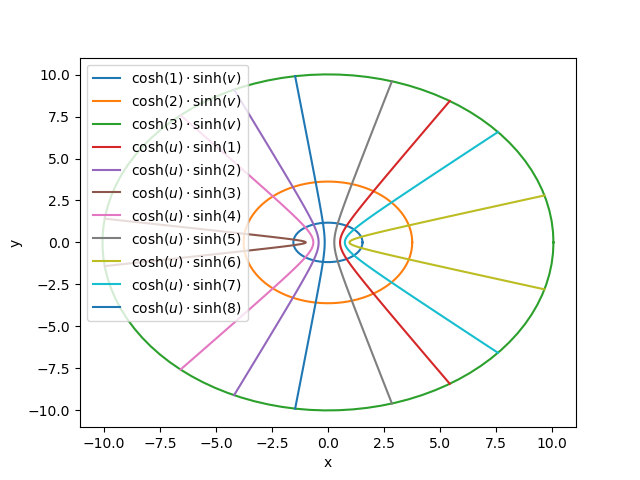
\includegraphics{2c.png}
	\end{figure}
	\newpage	
	\subsection*{d}
	Python kode til dette er
	\begin{lstlisting}
import numpy as np
import sympy as sp
import matplotlib.pyplot as plt

u, v = psi = sp.symbols("u, v", real=True)
r = (sp.cosh(u)*sp.cos(v), sp.sinh(u)*sp.sin(v))

def basisvektor(psi, r):
    b = np.zeros((len(psi), len(r)), dtype=object)
    for i, ui, in enumerate(psi):
        for j, rj in enumerate(r):
            b[i, j] = sp.simplify(rj.diff(ui, 1))
    return b

def skaleringsfaktor(b):
    h = np.zeros(b.shape[0], dtype=object)
    for i, s in enumerate(np.sum(b**2, axis=1)):
        h[i] = sp.simplify(sp.sqrt(s))
    return h

def enhetsvektor(psi, r):
    b = basisvektor(psi, r)
    hi = skaleringsfaktor(b)
    return b/ hi[None, :], hi

e, h = enhetsvektor(psi, r)

f = (1 - u**2)*sp.cos(2*v)

N = 100
ui = np.broadcast_to(np.linspace(0, 1, N)[:, None], (N, N))
vi = np.broadcast_to(np.linspace(0, 2*np.pi, N)[None, :], (N, N))
fj = sp.lambdify((u, v), f)(ui, vi)

mesh = []
for rj in r:
    mesh.append(sp.lambdify((u, v), rj)(ui, vi))
x, y = mesh

plt.contourf(x, y, fj)

df = np.array((1/h[0]*f.diff(u, 1), 1/h[1]*f.diff(v, 1)))

gradf = e[0]*df[0] + e[1]*df[1]

dfdxi = sp.lambdify((u, v), gradf[0])(ui, vi)
dfdyi = sp.lambdify((u, v), gradf[1])(ui, vi)
plt.contourf(x, y, fj)
plt.quiver(x[::50], y[::50], dfdxi[::50], dfdyi[::50], scale=15, pivot="middle")

plt.xlabel("x")
plt.ylabel("y")

plt.savefig("2d.png")
plt.show()
plt.close()

plt.contourf(ui, vi, fj)
plt.xlabel("x")
plt.ylabel("y")
plt.savefig("2d_elliptical.png")
plt.show()
	\end{lstlisting}
	\newpage
	\begin{figure}[h!]
		\centering
		\caption{Konturplott i elliptiske koordinater oppgave 2d}
		\label{fig:2d_elliptical}
		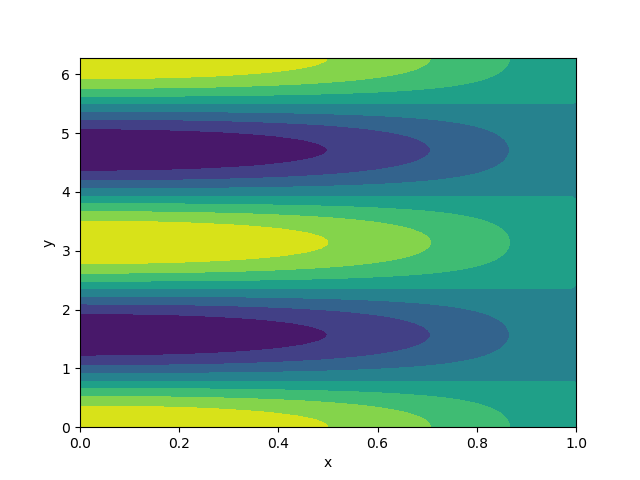
\includegraphics{2d_elliptical.png}
	\end{figure}
	
		\begin{figure}[h!]
			\centering
			\caption{Pilplott til oppgave 2d}
			\label{fig:2d}
			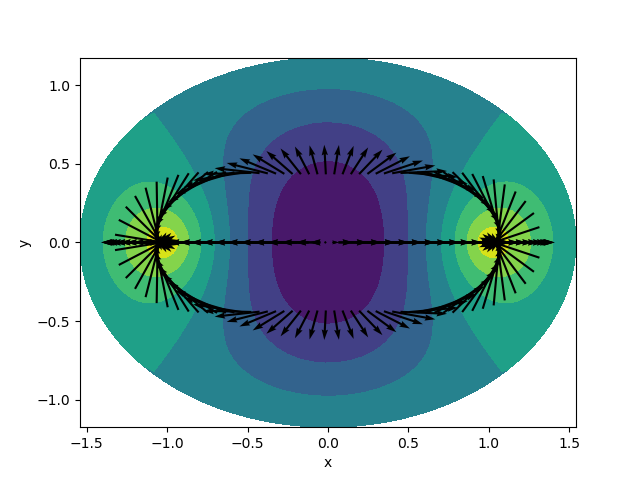
\includegraphics{2d.png}
		\end{figure}
		Observerer da at vektorene peker ut i fra origo og blir slukt ned i brennpunktene $(-1, 0)$ og $(1,0)$
		\newpage
	

\section*{3}
	\subsection*{a}
		Strømfunksjon \[
		v_x = \frac{\partial \psi}{\partial y}  \wedge v_y = \frac{\partial \psi}{\partial x} 
		\] 
		\begin{align*}
			& \frac{\partial \psi}{\partial y} = -v_x
			& \wedge &
			& \frac{\partial \psi}{\partial x} = v_y\\
			& \psi (x,y) = - \int \cos(x) \sin(y) \mathrm{e} ^{-2vt} \dd{y}
			& \wedge &
			& \psi (x,y) = \int -\sin(x) \cos(y) \mathrm{e}^{-2vt} \dd{x}\\
			& \psi (x,y) = - \cos(x) \cos(y)  \mathrm{e}^{-2vt} + C
			& \wedge &
			& \psi (x,y) = - \cos(x) \cos(y)  \mathrm{e}^{-2vt} + C
		\end{align*}
		Ser så om den har ett skalarpotensial. Hvis det har det så må 
		\begin{align*}
			&\frac{\partial \phi}{\partial x} = v_x 
			&\wedge & 
			&\frac{\partial \phi}{\partial y} = v_y \\
			& \phi(x,y) = \int \cos(x) \sin(y) \mathrm{e}^{-2vt} \dd{x}
			& \wedge &
			& \phi(x,y) = \int \left( -\sin(x) \cos(y) \mathrm{e}^{-2vt} \right) \dd{y}\\
			& \phi = \sin(x) \sin(y) \mathrm{e}^{-2vt} + f(y)
			& \wedge &
			& \phi = - \sin(x) \sin(y) \mathrm{e}^{-2vt} + f(x)
		\end{align*}
		Disse kan ikke være like så det finnes ikke noe skalarpotensial
	
	\subsection*{b}
		Python kode til pilplott med strømlinjer

		Som produserer følgende graf
		\begin{figure}[h!]
			\centering
			\caption{Pilplott med strømlinjer til 3b}
			\label{fig:3b}
			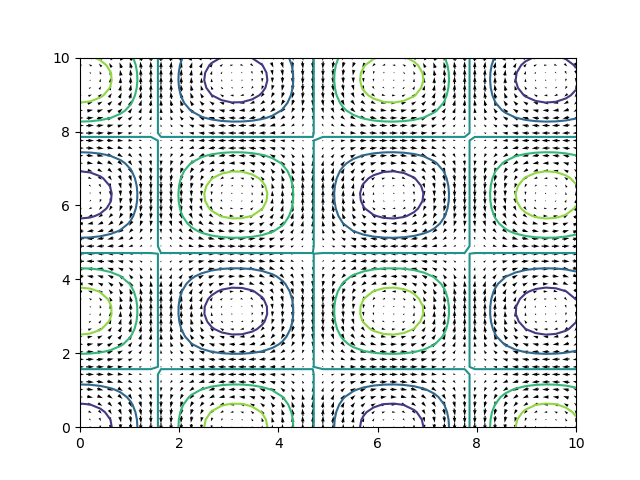
\includegraphics{3b.png}
		\end{figure}
		\newpage
		
	\subsection*{c}
		Kan bruke Gauss' divergensteorem siden det er en generalisering av Green Sett inn mer her siden 
		\begin{align*}
			\int\limits_C \vec{u}  \cdot \vec{n} \dd{s} = \iint \limits_R \nabla \cdot \vec{u} \dd{x}\dd{y}
		\end{align*}
		Regner ut $\nabla \cdot \vec{u} $ 
		\begin{align*}
			&\nabla \cdot \vec{u} = \frac{\partial }{\partial x} \left( \cos(x) \sin(y)  \right) + \frac{\partial }{\partial y} \left( -\sin(x) \cos(y)  \right) \\
			&\nabla \cdot \vec{u} = - \sin(x) \sin(y) + \sin(x) \sin(y) \\
			&\nabla \cdot \vec{u} = 0
		\end{align*}
		Følgelig er fluksen da $0$\\
		Sirkulasjonen blir da
		\begin{align*}
			&\oint \vec{u}  \cdot \dd{\vec{r} } = \int\limits_0^{\frac{\pi}{2}} \vec{u} \cdot \dd{\vec{r}_{x,0} } + \int\limits_0^{\frac{\pi}{2}} \vec{u} \cdot \dd{\vec{r}_{y,0} }+  \int\limits_{\frac{\pi}{2}}^0 \vec{u} \cdot \dd{\vec{r}_{x,1} } + \int\limits_{\frac{\pi}{2}}^0 \vec{u} \cdot  \dd{\vec{r}_{y,1} }\\
			&\boxed{%
				\begin{aligned}
				&\vec{r}_{x,0}(t') = t' \uvec{i} + 0 \uvec{j} &\wedge&  &\vec{r}_{y,0}(t') = \frac{\pi}{2} \uvec{i} + t' \uvec{j} 
				&\wedge&  &\vec{r}_{x,1}(t') = t' \uvec{i} + \frac{\pi}{2}\uvec{j} &\wedge & &\vec{r}_{y,1}(t') = 0 \uvec{i} + t' \uvec{j}\\
				&\overrightarrow{r}'_{x,0}(t') = \uvec{i} &\wedge & &\overrightarrow{r}'_{y,0}(t') = \uvec{j}
				&\wedge & & \overrightarrow{r}'_{x,1}(t') = \uvec{i} &\wedge & & \overrightarrow{r}_{y,1}^{\prime} (t') = \uvec{j}
			\end{aligned}}\\
			&\oint \vec{u}  \cdot \dd{\vec{r} } =  
			\begin{aligned}
				&\int\limits_0^{\frac{\pi}{2}} \vec{u} \left( \vec{r}_{x,0}(t')  \right) \cdot \overrightarrow{r}'_{x,0}(t') \dd{t'} 
				+ \int\limits_0^{\frac{\pi}{2}} \vec{u} \left( \vec{r}_{y,0}(t')  \right) \cdot \overrightarrow{r}'_{y,0}(t') \dd{t'}\\
				&+ \int\limits_{\frac{\pi}{2}}^0 \vec{u} \left( \vec{r}_{x,1}(t') \right) \cdot \overrightarrow{r}'_{x,1} \dd{t'}
				+\int\limits_{\frac{\pi}{2}}^0 \vec{u} \left( \vec{r}_{y,1}(t') \right) \cdot \overrightarrow{r}'_{y,1} \dd{t'}\\
			\end{aligned}
		\end{align*}
		For å få det litt mer oversiktelig så regner jeg ett integral av gangen. Starter med
		\begin{align*}
			&\int\limits_0^{\frac{\pi}{2}} \vec{u} \left( \vec{r}_{x,0}(t')  \right) \cdot \overrightarrow{r}'_{x,0}(t') \dd{t'} = 
			\int\limits_0^{\frac{\pi}{2}} \left( \cos(t')\sin(0) \mathrm{e}^{-2vt}  \right) \uvec{i}\cdot \uvec{i} \dd{t'}\\
			&\int\limits_0^{\frac{\pi}{2}} \vec{u} \left( \vec{r}_{x,0}(t')  \right) \cdot \overrightarrow{r}'_{x,0}(t') \dd{t'} = 
			\int\limits_0^{\frac{\pi}{2}} \left( \cos(t')\sin(0) \mathrm{e}^{-2vt}   \right) \dd{t'}\\
			&\int\limits_0^{\frac{\pi}{2}} \vec{u} \left( \vec{r}_{x,0}(t')  \right) \cdot \overrightarrow{r}'_{x,0}(t') \dd{t'} =
			\int\limts_0^{\frac{\pi}{2}} 0 \dd{t'}\\
			&\int\limits_0^{\frac{\pi}{2}} \vec{u} \left( \vec{r}_{x,0}(t')  \right) \cdot \overrightarrow{r}'_{x,0}(t') \dd{t'} = 0
		\end{align*}
		Ser så på
		\begin{align*}
			&\int\limits_0^{\frac{\pi}{2}} \vec{u} \left( \vec{r}_{y,0}(t')  \right) \cdot \overrightarrow{r}'_{y,0}(t') \dd{t'} =
			\int\limits_0^{\frac{\pi}{2}}\left( -\sin \left( \frac{\pi}{2} \right) \cos(t') \mathrm{e}^{-2vt}  \right)\uvec{j} \cdot \uvec{j}\dd{t'}\\
			&\int\limits_0^{\frac{\pi}{2}} \vec{u} \left( \vec{r}_{y,0}(t')  \right) \cdot \overrightarrow{r}'_{y,0}(t') \dd{t'} =
			\int\limits_0^{\frac{\pi}{2}}\left( -\sin \left( \frac{\pi}{2} \right) \cos(t') \mathrm{e}^{-2vt}  \right) \dd{t'}\\
			&\int\limits_0^{\frac{\pi}{2}} \vec{u} \left( \vec{r}_{y,0}(t')  \right) \cdot \overrightarrow{r}'_{y,0}(t') \dd{t'} =
			-\mathrm{e}^{-2vt} \int\limits_0^{\frac{\pi}{2}} \cos(t') \dd{t'}\\
			&\int\limits_0^{\frac{\pi}{2}} \vec{u} \left( \vec{r}_{y,0}(t')  \right) \cdot \overrightarrow{r}'_{y,0}(t') \dd{t'} =
			-\mathrm{e}^{-2vt} \left[ \sin(t') \right]\limits_0^{\frac{\pi}{2}}\\
			&\int\limits_0^{\frac{\pi}{2}} \vec{u} \left( \vec{r}_{y,0}(t')  \right) \cdot \overrightarrow{r}'_{y,0}(t') \dd{t'} = - \mathrm{e}^{-2vt} \left( 1 - 0 \right) \\
			&\int\limits_0^{\frac{\pi}{2}} \vec{u} \left( \vec{r}_{y,0}(t')  \right) \cdot \overrightarrow{r}'_{y,0}(t') \dd{t'} = - \mathrm{e}^{-2vt}
		\end{align*}
		Ser så på
		\begin{align*}
			&\int\limits_{\frac{\pi}{2}}^0 \vec{u} \left( \vec{r}_{x,1}(t') \right) \cdot \overrightarrow{r}'_{x,1} \dd{t'} = 
			\int\limits_{\frac{\pi}{2}}^0 \left( \cos(t') \sin\left (\frac{\pi}{2} \right)  \right) \uvec{i} \cdot \uvec{i} \dd{t'}\\
			&\int\limits_{\frac{\pi}{2}}^0 \vec{u} \left( \vec{r}_{x,1}(t') \right) \cdot \overrightarrow{r}'_{x,1} \dd{t'} =
			\mathrm{e}^{-2vt}\int\limits_{\frac{\pi}{2}}^0 \cos(t') \dd{t'}\\ 
			&\int\limits_{\frac{\pi}{2}}^0 \vec{u} \left( \vec{r}_{x,1}(t') \right) \cdot \overrightarrow{r}'_{x,1} \dd{t'} =
			\mathrm{e}^{-2vt} \left[ \sin(t') \right]\limits_{\frac{\pi}{2}}^0\\
			&\int\limits_{\frac{\pi}{2}}^0 \vec{u} \left( \vec{r}_{x,1}(t') \right) \cdot \overrightarrow{r}'_{x,1} \dd{t'} =
			\mathrm{e}^{-2vt} \left( 0-1 \right) \\
			&\int\limits_{\frac{\pi}{2}}^0 \vec{u} \left( \vec{r}_{x,1}(t') \right) \cdot \overrightarrow{r}'_{x,1} \dd{t'} =
			-\mathrm{e}^{-2vt}
		\end{align*}
		Ser så på
		\begin{align*}
			&\int\limits_{\frac{\pi}{2}}^0 \vec{u} \left( \vec{r}_{y,1}(t') \right) \cdot \overrightarrow{r}'_{y,1} \dd{t'} = 
			\int\limits_{\frac{\pi}{2}}^0 \left( -\sin(0) \cos(t') \mathrm{e}^{-2vt}  \right) \uvec{j} \cdot \uvec{j} \dd{t'}\\
			&\int\limits_{\frac{\pi}{2}}^0 \vec{u} \left( \vec{r}_{y,1}(t') \right) \cdot \overrightarrow{r}'_{y,1} \dd{t'} =
			\int\limits_{\frac{\pi}{2}}^0 \left( -\sin(0) \cos(t') \mathrm{e}^{-2vt}  \right) \dd{t'}\\
			&\int\limits_{\frac{\pi}{2}}^0 \vec{u} \left( \vec{r}_{y,1}(t') \right) \cdot \overrightarrow{r}'_{y,1} \dd{t'} =
			\int\limits_{\frac{\pi}{2}}^0 0 \dd{t'}\\
			&\int\limits_{\frac{\pi}{2}}^0 \vec{u} \left( \vec{r}_{y,1}(t') \right) \cdot \overrightarrow{r}'_{y,1} \dd{t'} = 0
		\end{align*}
		Kan så gå tilbake til sirkulasjonen
		\begin{align*}
			&\oint \vec{u}  \cdot \dd{\vec{r} } = 0  - \mathrm{e}^{-2vt} - \mathrm{e}^{-2vt} + 0 = -2 \mathrm{e}^{-2vt}
		\end{align*}
		Kan også bruke Stokes sats som sier \[
			\oint\limts_C \vec{u} \cdot \dd{\vec{r}} = \int\limits_\sigma \left( \nabla \times \vec{u}  \right) \cdot \vec{n} \dd{\sigma}
		\] 
		Der 
		\begin{align*}
			& \nabla \times \vec{u} =
			\begin{vmatrix}
				\uvec{i} &\uvec{j} & \uvec{k}\\
				\frac{\partial }{\partial x} & \frac{\partial }{\partial y} & \frac{\partial }{\partial z} \\
				\cos(x) \sin(y) \mathrm{e}^{-2vt} & - \sin(x) \cos(y) \mathrm{e}^{-2vt} & 0
			\end{vmatrix}\\
			& \nabla \times \vec{u} = \mathrm{e}^{-2vt}\left( \frac{\partial }{\partial x} \left( -\sin(x) \cos(y)  \right) - \frac{\partial }{\partial y} \left( \cos(x) \sin(y)  \right)  \right)  \uvec{k}\\
			& \nabla \times \vec{u} = \mathrm{e}^{-2vt}\left( - \cos(x) \cos(y)  - \cos(x) \cos(y)  \right) \uvec{k}\\
			& \nabla \times \vec{u} = -2\mathrm{e}^{-2vt} \cos(x) \cos(y) \uvec{k}
		\end{align*}
		Og $\vec{n} = \uvec{k}$ siden den har positiv orientering om $z$. Da blir Stokes
		 \begin{align*}
			 &\int\limits_ \sigma \left( \nabla \times \vec{u}  \right) \cdot \vec{n} \dd{\sigma} = \int\limits_ \sigma \left( -2 \mathrm{e}^{-2vt}\cos(x) \cos(y)   \right)\uvec{k} \cdot \uvec{k} \dd{\sigma} \\
			 &\int\limits_ \sigma \left( \nabla \times \vec{u}  \right) \cdot \vec{n} \dd{\sigma} =-2 \mathrm{e}^{-2vt} \int\limits_ \sigma\left( \cos(x) \cos(y)   \right) \dd{\sigma}\\
			 &\int\limits_ \sigma \left( \nabla \times \vec{u}  \right) \cdot \vec{n} \dd{\sigma} = -2 \mathrm{e}^{-2vt} \int\limits_0^{\frac{\pi}{2}} \int\limits_0^{\frac{\pi}{2}}\cos(x) \cos(y) \dd{x}\dd{y}\\
			 &\int\limits_ \sigma \left( \nabla \times \vec{u}  \right) \cdot \vec{n} \dd{\sigma} =-2 \mathrm{e}^{-2vt} \int\limits_0^{\frac{\pi}{2}}\cos(y) \left[\sin(x) \right]\limits_0^{\frac{\pi}{2}} \dd{y}\\
			 &\int\limits_ \sigma \left( \nabla \times \vec{u}  \right) \cdot \vec{n} \dd{\sigma} =-2 \mathrm{e}^{-2vt} \int\limits_0^{\frac{\pi}{2}}\cos(y) \left( 1-0 \right) \dd{y}\\
			 &\int\limits_ \sigma \left( \nabla \times \vec{u}  \right) \cdot \vec{n} \dd{\sigma} =-2 \mathrm{e}^{-2vt} \int\limits_0^{\frac{\pi}{2}}\cos(y) \dd{y}\\
			 &\int\limits_ \sigma \left( \nabla \times \vec{u}  \right) \cdot \vec{n} \dd{\sigma} =-2 \mathrm{e}^{-2vt}\left[\sin(y) \right]\limits_0^{\frac{\pi}{2}}\\
			 &\int\limits_ \sigma \left( \nabla \times \vec{u}  \right) \cdot \vec{n} \dd{\sigma} =-2 \mathrm{e}^{-2vt}\left( 1-0 \right) \\
			 &\int\limits_ \sigma \left( \nabla \times \vec{u}  \right) \cdot \vec{n} \dd{\sigma} =-2 \mathrm{e}^{-2vt}
		\end{align*}
	\subsection*{d}
	Setter $x(t) = \cos(t) $ og $y(t)=\sin(t) $ da blir \[
		z(t) = \cos(\cos(t) ) \cos(\sin(t) ) 
	\] 
	Deriverer vi $x,y$ med hensyn på $t$ får vi da
	\begin{align*}
		&x'(t)	= - \sin(t) &\wedge & &y'(t) = \cos(t) 
	\end{align*}
	og $z$
	 \begin{align*}
		 &z'(t) = \frac{\dd{}}{\dd{t}} \left( \cos(\cos(t) ) \cos(\sin(t) )  \right) \\
		 &z'(t) = \cos(\sin(t) ) \frac{\dd{}}{\dd{t}}\left ( \cos(\cos(t) )\right) + \cos(\cos(t) ) \frac{\dd{}}{\dd{t}}\left ( \cos(\sin(t) )\right) \\
		 &\boxed{u = \cos(t) \wedge v = \sin(t) }\\
		 &z'(t) = \cos(\sin(t) ) \frac{\dd{}}{\dd{u}}\left( \cos(u)  \right) \frac{\dd{}}{\dd{t}}\left( \cos(t)  \right) + \cos(\cos(t) ) \frac{\dd{}}{\dd{v}} \left( \cos(v)  \right) \frac{\dd{}}{\dd{t}} \sin(t) \\
		 &z'(t) = \cos(\sin(t) ) \left( - \sin(u)  \right) \left( -\sin(t)  \right) + \cos(\cos(t) ) \left( - \sin(v)  \right) \cos(t)  \\
		 &z'(t) = \cos(\sin(t) ) \sin(\cos(t) ) \sin(t)  - \cos(\cos(t)) \sin(\sin(t) ) \cos(t) 
	\end{align*}
	For å finne buelengden så kan man bruke formelen \[
		L(a,b) = \int\limits_a^b \sqrt{\left( x'(t) \right) ^2 + \left( y'(t) \right) ^2 + \left( z'(t) \right) ^2} \dd{t}
	\] 
	Der $a=0$ og $b= 2 \pi$ så blir integrallet
	\begin{align*}
		\int\limits_0^{2 \pi} \sqrt{\left( - \sin(t)  \right)^2 + \left( \cos(t)  \right) ^2 + \left(\cos(\sin(t) ) \sin(\cos(t) ) \sin(t)  - \cos(\cos(t)) \sin(\sin(t) ) \cos(t)  \right)^2 }\dd{t}
	\end{align*}
	Bruker Python til å regne ut det integrallet og koden ser slik ut
	\begin{lstlisting}
import numpy as np

t = np.linspace(0, 2*np.pi, 1000)

dx = -np.sin(t)
dy = np.cos(t)
dz = np.cos(np.cos(t))*np.sin(np.cos(t))*np.sin(t) - np.cos(np.cos(t))*np.sin(np.sin(t))*np.cos(t)

L = np.trapz(np.sqrt(dx**2 + dy**2 + dz**2), t)

print(f"{L:f}")
	\end{lstlisting}
	Som gir meg at \[
	L = 6.284694
	\] 
	Som er litt større enn $2 \pi$ som gir mening siden kurven ser noe slikt ut i Geogebra
	\begin{figure}[h!]
		\centering
		\caption{Kurven til 3d}
		\label{fig:3d}
		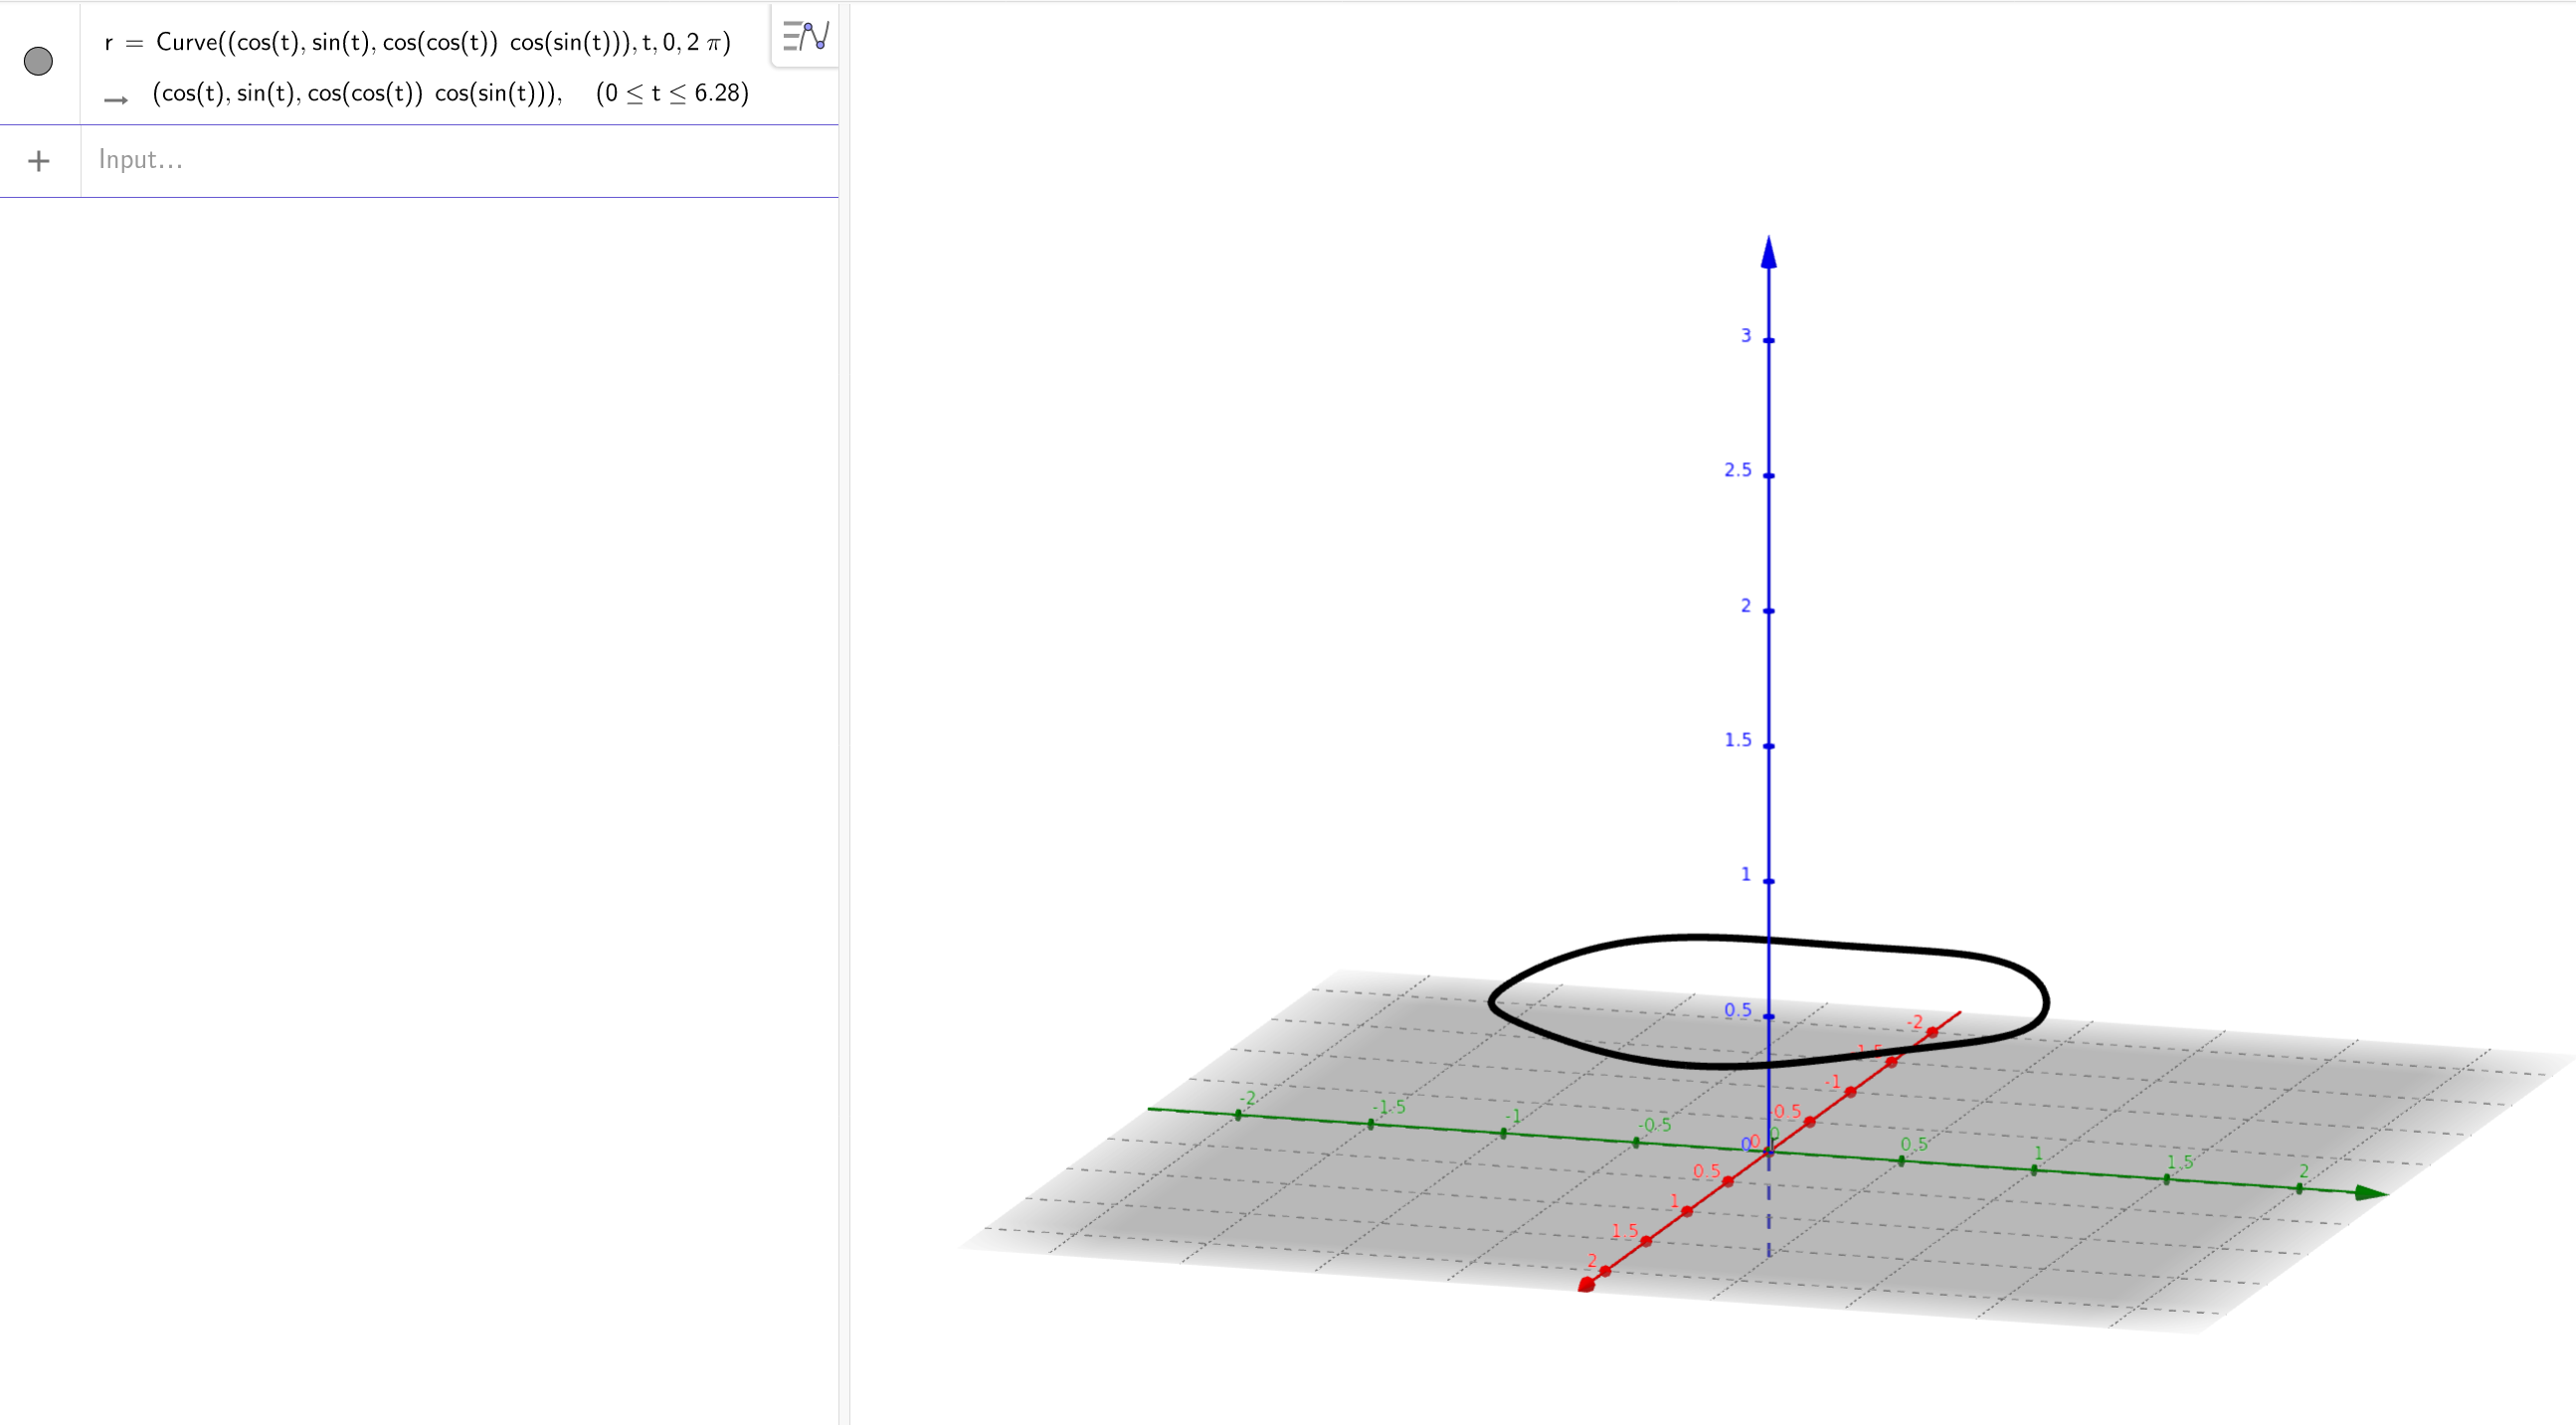
\includegraphics[scale=0.18]{3d.png}
	\end{figure}
	\newpage
	\subsection*{e}
		Bruker formelen \[
		\frac{D \vec{v} }{D t} = \frac{\partial \vec{v} }{\partial t}  + \vec{v} \cdot \nabla \vec{v} 
		\] 
		Der $\vec{v} = \vec{u} = \left( \cos(x) \sin(y) \uvec{i} - \sin(x) \cos(y) \uvec{j} \right) \mathrm{e}^{-2vt} $\\
		Finner først lokalakselerasjonen
		\begin{align*}
			&\frac{\partial \vec{u} }{\partial t} = \frac{\partial }{\partial t} \left( \cos(x) \sin(y) \uvec{i} - \sin(x) \cos(y) \uvec{j} \right) \mathrm{e}^{-2vt}\\
			&\frac{\partial \vec{u} }{\partial t} = \left( \cos(x) \sin(y) \uvec{i} - \sin(x) \cos(y) \uvec{j} \right) \frac{\partial }{\partial t} \mathrm{e}^{-2vt}\\ 
			&\frac{\partial \vec{u} }{\partial t} = -2v\left( \cos(x) \sin(y) \uvec{i} - \sin(x) \cos(y) \uvec{j} \right)\mathrm{e}^{-2vt}\\
			&\frac{\partial \vec{u} }{\partial t} = -2v \vec{u} 
		\end{align*}
		Finner så den konvektive akselerasjonen
		\begin{align*}
			&\vec{u} \cdot \nabla \vec{u} = \left( \vec{u}  \cdot \nabla u_x \right) \uvec{i} + \left( \vec{u} \cdot \nabla u_y \right) \uvec{j}\\
			&\vec{u} \cdot \nabla \vec{u} = u_x \frac{\partial \vec{u} }{\partial x} + u_y \frac{\partial \vec{u} }{\partial y} \\
			&\vec{u} \cdot \nabla \vec{u} = u_x \frac{\partial }{\partial x} \left(\left( \cos(x) \sin(y) \uvec{i} - \sin(x) \cos(y) \uvec{j} \right) \mathrm{e}^{-2vt}  \right) 
			+ u_y  \frac{\partial }{\partial y} \left( \left( \cos(x) \sin(y) \uvec{i} - \sin(x) \cos(y) \uvec{j} \right) \mathrm{e}^{-2vt} \right) \\
			&\vec{u} \cdot \nabla \vec{u} = \mathrm{e}^{-2vt} \left( u_x \left( -\sin(x) \sin(y) \uvec{i} - \cos(x) \cos(y) \uvec{j} \right) 
			+ u_y \left( \cos(x) \cos(y) \uvec{i} + \sin(x) \sin(y) \uvec{j} \right)  \right) \\
			&\vec{u} \cdot \nabla \vec{u} = \mathrm{e}^{-2vt} 
			\begin{aligned}
				\Bigg( &\cos(x) \sin(y) \mathrm{e}^{-2vt} \left( - \sin(x) \sin(y) \uvec{i} - \cos(x) \cos(y) \uvec{j}  \right) \\
				&- \sin(x) \cos(y) \mathrm{e}^{-2vt} \left( \cos(x) \cos(y) \uvec{i} + \sin(x) \sin(y) \uvec{j} \right)   \Bigg) 
			\end{aligned}\\
			&\vec{u} \cdot \nabla \vec{u} = \mathrm{e}^{-4vt} \left( \cos(x) \sin(y) \left( -\sin(x) \sin(y) \uvec{i} - \cos(x) \cos(y) \uvec{j} \right) 
			- \sin(x) \cos(y) \left( \cos(x) \cos(y) \uvec{i} - \sin(x) \sin(y) \uvec{j} \right) \right) \\
			&\vec{u} \cdot \nabla \vec{u} =\mathrm{e}^{-4vt} \left( -\sin^2 \left( y \right)\cos(x) \sin(x)  \uvec{i} - \cos^2 \left( x \right) \cos(y) \sin(y) \uvec{j} 
			- \cos^2 \left( y \right) \cos(x) \sin(x) \uvec{i} - \sin^2 \left( x \right) \cos(y) \sin(y) \uvec{j}\right) \\
			&\vec{u} \cdot \nabla \vec{u} =\mathrm{e}^{-4vt}
			\begin{aligned}
				&\Bigg( - \left( \left( \sin^2 \left( y \right) \cos(x) \sin(x) + \cos^2 \left( y \right) \cos(x) \sin(x)  \right) \uvec{i}\\
				&+ \left( \cos^2 \left( x \right) \cos(y) \sin(y)  + \sin^2 \left( x \right) \cos(y) \sin(y)  \right) \uvec{j}\Big)  \Bigg) 
			\end{aligned}\\
			&\vec{u} \cdot \nabla \vec{u} =-\mathrm{e}^{-4vt} \left( \cos(x) \sin(x) \left( \sin^2 \left( y \right) + \cos^2 \left( y \right)  \right) \uvec{i}
			+\cos(y) \sin(y) \left( \sin^2 \left( x \right) +\cos^2 \left( x \right)  \right) \uvec{j}\right) \\
			&\boxed{\sin^2 \left( x \right) + \cos^2 \left( x \right) = 1}\\
			&\vec{u} \cdot \nabla \vec{u} =-\mathrm{e}^{-4vt} \left( \cos(x) \sin(x) \uvec{i} + \cos(y) \sin(y) \uvec{j} \right) \\
			&\boxed{2 \cos(x) \sin(x) = \sin(2x) }\\
			&\vec{u} \cdot \nabla \vec{u} =-\mathrm{e}^{-4vt} \left( \frac{1}{2}\sin(2x) \uvec{i} + \frac{1}{2}\sin(2y) \uvec{j} \right) \\
			&\vec{u} \cdot \nabla \vec{u} = - \frac{1}{2}\mathrm{e}^{-4vt} \left( \sin(2x) \uvec{i} + \sin(2y) \uvec{j} \right) 
		\end{align*}
		Da blir \[
			\frac{D \vec{u} }{D t} = - 2v \vec{u}  - \frac{1}{2}\left( \sin(2x) \uvec{i} + \sin(2y) \uvec{j} \right) \mathrm{e}^{-4vt}_\blacksquare
		\] 
		Skal så finne trykket $p$ 
		\begin{align*}
			\frac{D \vec{u} }{D t} &= - \nabla p + v \nabla^2 \vec{u} \\
			\nabla p &= v \nabla^2 \vec{u} - \frac{D \vec{u} }{D t}\\
			\nabla p &= v \nabla^2 \vec{u}  + 2v \vec{u} + \frac{1}{2} \left( \sin(2x) \uvec{i} + \sin(2y) \uvec{j} \right) \mathrm{e}^{-4vt}
		\end{align*}
		Må først da regne ut
		\begin{align*}
			& v \cdot \nabla^2 \vec{u} = v \cdot \left( \frac{\partial ^2}{\partial x^2} \vec{u} + \frac{\partial ^2}{\partial y^2} \vec{u}  \right) \\
			&\boxed{%
				\begin{aligned}
					&\frac{\partial ^2}{\partial x^2} \vec{u} = \frac{\partial ^2}{\partial x^2 } \left( \cos(x) \sin(y) \uvec{i} - \sin(x) \cos(y) \uvec{j} \right) \mathrm{e}^{-2vt}\\ 
					&\frac{\partial ^2}{\partial x^2} \vec{u} = \frac{\partial }{\partial x} \left( -\sin(x) \sin(y) \uvec{i} - \cos(x) \cos(y) \uvec{j} \right) \mathrm{e}^{-2vt}\\
					& \frac{\partial ^2}{\partial x^2} \vec{u} = \left(- \cos(x)\sin(y) \uvec{i} + \sin(x) \cos(y) \uvec{j}  \right) \mathrm{e}^{-2vt}
			\end{aligned}}\\
			&\boxed{%
				\begin{aligned}
					&\frac{\partial ^2}{\partial y^2} \vec{u} = \frac{\partial ^2}{\partial y^2 } \left( \cos(x) \sin(y) \uvec{i} - \sin(x) \cos(y) \uvec{j} \right) \mathrm{e}^{-2vt}\\ 
					&\frac{\partial ^2}{\partial y^2} \vec{u} = \frac{\partial }{\partial y} \left( \cos(x) \cos(y) \uvec{i} + \sin(x) \sin(y) \uvec{j} \right) \mathrm{e}^{-2vt}\\
					& \frac{\partial ^2}{\partial y^2} \vec{u} = \left(- \cos(x) \sin(y) \uvec{i} + \sin(x) \cos(y) \uvec{j}  \right) \mathrm{e}^{-2vt}
			\end{aligned}}\\
			& v \cdot \nabla^2 \vec{u} = v \cdot \left ( \left(- \cos(x)\sin(y) \uvec{i} + \sin(x) \cos(y) \uvec{j}  \right) \mathrm{e}^{-2vt}
			\cdot \left(- \cos(x) \sin(y) \uvec{i} + \sin(x) \cos(y) \uvec{j}  \right) \mathrm{e}^{-2vt} \right)\\
			& v \cdot \nabla^2 \vec{u} = v \mathrm{e}^{-2vt} \cdot \left( -2 \cos(x) \sin(y) \uvec{i} + 2 \sin(x) \cos(y) \uvec{j} \right) \\
			& v \cdot \nabla^2 \vec{u} =-2v \left(\cos(x) \sin(y) \uvec{i} - \sin(x) \cos(y) \uvec{j}  \right)  \mathrm{e}^{-2vt}\\
			& v \cdot \nabla^2 \vec{u} = - 2v \vec{u} 
		\end{align*}
		Da blir \[
		\nabla p =2v \vec{u} + \frac{1}{2} \left( \sin(2x) \uvec{i} + \sin(2y) \uvec{j} \right) \mathrm{e}^{-4vt} - 2v \vec{u} 
		\] 
		Ser så på integrallet med hensyn på $x$ 
		\begin{align*}
			&p(x,y,t) = \int \left( 2v \vec{u} + \frac{1}{2} \left( \sin(2x) \uvec{i} + \sin(2y) \uvec{j} \right) \mathrm{e}^{-4vt} - 2v \vec{u} \right) \dd{x}
		\end{align*}
		Tar integrallene hver for seg
		\begin{align*}
			&\int 2v \vec{u} \dd{x} = 2v \int \left( \cos(x) \sin(y) \uvec{i} - \sin(x) \cos(y) \uvec{j} \right) \mathrm{e}^{-2vt} \dd{x}\\
			&\int 2v \vec{u} \dd{x} = 2v \mathrm{e}^{-2vt} \left( - \sin(x) \sin(y) \uvec{i} - \cos(x) \cos(y) \uvec{j} \right) \\
		\end{align*}
		Ser så på
		\begin{align*}
			&\int \frac{1}{2}\left( \sin(2x) \uvec{i} + \sin(2y) \uvec{j} \right) \mathrm{e}^{-4vt} \dd{x} = \frac{1}{2}\mathrm{e}^{-4vt} \int \left( \sin(2x) \uvec{i} + \sin(2y) \uvec{j} \right) \dd{x}\\
			&\int \frac{1}{2}\left( \sin(2x) \uvec{i} + \sin(2y) \uvec{j} \right) \mathrm{e}^{-4vt} \dd{x} = \frac{1}{2} \mathrm{e}^{-4vt} \cdot \left( - \frac{1}{2}\cos(2x) \uvec{i} \right) \\
			&\int \frac{1}{2}\left( \sin(2x) \uvec{i} + \sin(2y) \uvec{j} \right) \mathrm{e}^{-4vt} \dd{x} = - \frac{1}{4}\mathrm{e}^{-4vt} \cos(2x) \uvec{i}
		\end{align*}
		Observerer at det første og siste integrallet er likt bare med motsatt fortegn \[
			&\int- 2v \vec{u} \dd{x} = -2v \mathrm{e}^{-2vt} \left( - \sin(x) \sin(y) \uvec{i} - \cos(x) \cos(y) \uvec{j} \right) \\
		\] 
		Da blir
		\begin{align*}
			&p(x,y,t) =
			\begin{aligned}
			&2v \mathrm{e}^{-2vt} \left( - \sin(x) \sin(y) \uvec{i} - \cos(x) \cos(y) \uvec{j} \right) - \frac{1}{4}\mathrm{e}^{-4vt}\cos(2x) \uvec{i}\\
			&-2v \mathrm{e}^{-2vt} \left( - \sin(x) \sin(y) \uvec{i} - \cos(x) \cos(y) \uvec{j} \right) + f(y)\\
			\end{aligned}\\
			&p(x,y,t) = - \frac{1}{4}\mathrm{e}^{-4vt}\cos(2x) \uvec{i} + f(y)
		\end{align*}
		Ser så med hensyn på $y$ \[
			p(x,y,t) = \int \left( 2v \vec{u} + \frac{1}{2} \left( \sin(2x) \uvec{i} + \sin(2y) \uvec{j} \right) \mathrm{e}^{-4vt} - 2v \vec{u} \right) \dd{y}
		\] 
		Tar integrallene hver for seg
		\begin{align*}
			&\int 2v \vec{u} \dd{y} = 2v \int \left( \cos(x) \sin(y) \uvec{i} - \sin(x) \cos(y) \uvec{j} \right) \mathrm{e}^{-2vt} \dd{y}\\
			&\int 2v \vec{u} \dd{y} = 2v \mathrm{e}^{-2vt} \left( \cos(x)  \cos(y) \uvec{i} + \sin(x) \sin(y) \uvec{j} \right) \\
		\end{align*}
		Ser så på
		\begin{align*}
			&\int \frac{1}{2}\left( \sin(2x) \uvec{i} + \sin(2y) \uvec{j} \right) \mathrm{e}^{-4vt} \dd{y} = \frac{1}{2}\mathrm{e}^{-4vt} \int \left( \sin(2x) \uvec{i} + \sin(2y) \uvec{j} \right) \dd{y}\\
			&\int \frac{1}{2}\left( \sin(2x) \uvec{i} + \sin(2y) \uvec{j} \right) \mathrm{e}^{-4vt} \dd{y} = \frac{1}{2} \mathrm{e}^{-4vt} \cdot \left( - \frac{1}{2}\cos(2y) \uvec{j} \right) \\
			&\int \frac{1}{2}\left( \sin(2x) \uvec{i} + \sin(2y) \uvec{j} \right) \mathrm{e}^{-4vt} \dd{y} = - \frac{1}{4}\mathrm{e}^{-4vt} \cos(2y) \uvec{j}
		\end{align*}
		Observerer at det første og siste integrallet er likt bare med motsatt fortegn \[
			&\int- 2v \vec{u} \dd{y} = -2v \mathrm{e}^{-2vt} \left( \cos(x)  \cos(y) \uvec{i} + \sin(x) \sin(y) \uvec{j} \right) \\
		\] 
		Da blir
		\begin{align*}
			&p(x,y,t) =
			\begin{aligned}
			&2v \mathrm{e}^{-2vt} \left( - \sin(x) \sin(y) \uvec{i} - \cos(x) \cos(y) \uvec{j} \right) - \frac{1}{4}\mathrm{e}^{-4vt}\cos(2y) \uvec{j}\\
			&-2v \mathrm{e}^{-2vt} \left( - \sin(x) \sin(y) \uvec{i} - \cos(x) \cos(y) \uvec{j} \right) + g(x)\\
			\end{aligned}\\
			&p(x,y,t) = - \frac{1}{4}\mathrm{e}^{-4vt}\cos(2y) \uvec{j} + g(x)
		\end{align*}
		Sammenligner jeg disse 2 $p$-ene så ser jeg at \[
			g(x) = - \frac{1}{4}\mathrm{e}^{-4vt}\cos(2x) \uvec{i} \wedge f(y) =- \frac{1}{4}\mathrm{e}^{-4vt}\cos(2y) \uvec{j}
		\] 
		Følgelig blir \[
			p(x,y,t) =- \frac{1}{4}\mathrm{e}^{-4vt}\cos(2x) \uvec{i} - \frac{1}{4}\mathrm{e}^{-4vt}\cos(2y) \uvec{j}= - \frac{1}{4}\mathrm{e}^{-2vt} \left( \cos(2x) \uvec{i} + \cos(2y) \uvec{j} \right) 
		\] 
\end{document}
